\begin{landscape}
\begin{table}[t!]
    \caption{Observational study subjects - Data reflect the state of repositories as of 26 January 2015}
    \label{tab:subjects}
    %\multirow{2}{*}{Safety hole} & \multicolumn{2}{c}{Number of exported functions collected in the } \\
\centering
\resizebox{\linewidth}{!}{
\begin{tabular}{rlccccc}
    Project Name & Description & \# Files & \# Commits & \# Developers & \# Issues & \# Resolved Issues \\
\toprule
%{\tt Camel} & Integration framework& 22,655 & 18,684& 143& 8,250& 7,697 \\
%{\tt Cassandra} & Distributed database management system& 3,847 & 15,817 & 130 & 3,800& 3,087\\
{\tt Commons-codec} & General encoding/decoding algorithms & 635 & 1,424 & 24 & 195 & 177 \\
{\tt Commons-collections} & Extension of the Java Collections Framework& 2,983 & 2,722& 47 & 542 & 512\\
{\tt Commons-compress} & Library for working with file compression& 619 & 1,716& 24 & 308 & 272\\
{\tt Commons-csv} & Extension of the Java Collections Framework& 141 & 956& 18 & 147 & 119\\
{\tt Commons-io} & Collection of utilities for CSV file reading/writing & 631 & 1,718& 33 & 454 & 365\\
{\tt Commons-lang} & Extra-functionality for java.lang& 1,294 & 4,103& 46 & 1,073& 933\\
{\tt Commons-math} & Mathematics \& Statistics components & 4,582 & 5,496& 37 & 1,194& 1,085\\
%{\tt Hadoop} & Big data framework for distributed storage and processing & 22,722 & 9,800 & 104 & 9,525 & 7,938\\
{\tt Spring-framework} & Application framework for the Java platform& 19,721 & 9,748& 153& 3,500 & 2,632 \\
{\tt Storm} & Distributed real-time computation system& 2,038 & 3,534 & 189 & 637 & 321 \\
{\tt Wildfly} & aka JBoss Application Server& 31,699 &  16,855 & 307& 3,710 & 2,993\\
\midrule
{\tt Total} & & 64,388 & 48,272 & 878 & 11,760 & 9,409\\
%{\tt Total} & & 87,160 & 58,072 & 982 & 21,285 & 17,347\\
%{\tt Total} & & 113,662 & 92,573 & 1,255 & 33,335 & 281,313\\
\bottomrule
\end{tabular}
}

\end{table}
\end{landscape}

\section{Post-mortem Analysis for IC{\scriptsize s}}
\label{sec:preliminary}
In this study, we focus on systematically discovering influential
changes.  Although the motivating examples described in
Section~\ref{sec:motivation} show some intuitions on influential
changes, it is necessary to reveal a larger view to figure out the
characteristics of these changes. Therefore, we collected
\numChanges changes from
\numSubjects popular open-source projects and conducted an observational study.

%\begin{table*}[!t]
%\centering
%\caption{Subjects used in our observational study.  ``\# Commits'' is
%  the number of all change commits in the source code
%  repositories. ``\# Files'' is the total number of files included the
%  commits.\dongsun{Daoyuan, the number of unique files?} and ``\#
%  Committers'' is the number of developers\dongsun{Daoyuan, unique?}
%  who made changes.  ``\# Issues'' is the number of issues collected
%  from the corresponding issue tracking systems (ITS) of the projects
%  while ``\# Resolved'' represents the number of issues marked as
%  ``RESOLVED'' in ITS.  \todo{we need to migrate csv-tavular into
%    native table at the final stage!}  \todo{new row required:
%    ``total''}}
%\label{tab:subjects}
%\csvautotabular{table/overview.csv}
%\end{table*}

Since there are too many changes in software repositories and it is not
possible for us to inspect all, we get a set of changes that are likely to
have a higher density of influential changes. We are able to get this set by
leveraging several intuitions obtained from examples described in
Section~\ref{sec:motivation}.

The study design basically addressed three different criteria to
discover influential changes: 1) popular changes in the sense that they
have been somehow noticed by other developers and users,
2) anomalies in change behaviors, and 3) changes that are related to controversial/popular issues. 
These criteria are designed to conduct post-mortem analysis and represent how people
can recognize influential changes in hindsight.

For changes in these categories, we manually examine them using the following
procedure:
\begin{itemize}
	\item First of all, authors of this article ask themselves individually whether a change is really influential.
	They manually verify that the assumptions behind the specific criteria used to identify a change are supported.
	\item Then we cross-check the answers to reach a consensus among the authors.
\item Afterwards, we double check that these changes are really influential in
the eyes of developers by doing card sorting and surveying professional
developers.
\end{itemize}


% \tb{Sentence missing to say how we came up with these criteria. What gave us
% the intuitions? Previous examples from Section 2?}

\subsection{Data Collection}
The experiment subjects in this study are shown in 
Table~\ref{tab:subjects}. The \numSubjects popular
projects were considered since they have sufficient number of 
changes in their revision histories. In addition,
these projects stably maintained their issue tracking systems so that we
could keep track of how developers discussed to make software changes.


For each subject, we collected all available change data (patches and relevant
files information) as well as commit metadata (change date and author details) from
the source code repository.
Additionally, issue reports from the corresponding issue tracking system were
collected together. We further mined issue linking information from commit
messages and issue reports wherever possible: e.g., many commit messages
explicitly refer to the unique ID of the issue they are addressing, whether a
bug or a feature request.

\subsection{Systematic Analysis}
\label{sec:systemanalysis}
To systematically discover potential influential changes among the changes collected from
the subject projects, we propose to build on common intuitions about how a single change can
be influential in the development of a software project.

%\newpage
\subsubsection{Changes that address controversial/popular issues.}
\label{sec:blocking}
In software projects, developers use issue tracking systems
to track and fix bugs and for planning
future improvements. When an issue is reported, developers and/or
users may provide insights of how the issue can be investigated. 
Attempts to resolve the issue are also often recorded in the issue tracking
system.

Since an issue tracking system appears as an important place to discuss
about software quality, we believe it is natural to assume that heated
discussions about a certain issue may suggest the importance of this
specific issue. Furthermore, when an issue is finally resolved after an exceptionally
lengthy discussion, all early fix attempts and the final commit that resolves
the issue should be considered to be influential. Indeed all these
software changes have contributed to close the discussion, unlock whatever
has been blocking attention from other issues, and satisfy the majority of
stakeholders. 

To identify controversial/popular issues in projects, we first searched for
issues with an overwhelmingly larger number of comments than others within the
same project. In this study, we regarded an issue as a controversial/popular issue if the
number of its comments is larger than the 99th percentile of issue comment
numbers. Applying this simple criteria, we could identify a set of issues that
 are controversial/popular. Afterwards, we collected all commits that were
associated to each of the controversial/popular issues and tag them as potentially
influential.

% For example, in Hadoop we found that each issue was associated with 11
% comments on average. We were able to discover an influential change associated
% with issue HADOOP-10607 which generated over 70 comments. Developers and users
% spent over 1 month discussing the need (and the proper way) for eliminating
% the storage of passwords and secrets in clear text within configuration or
% source code files. The commit\footnote{Commit \tt\small
% c79728478caadd8374bce2bc3f466db1da1e3ad1} that resolved this issue provided a
% change in the form of a new API that now separates credential/password storage
% from applications.


An example was found in Apache Math. An
issue\footnote{Bug report \url{https://issues.apache.org/jira/browse/MATH-650}} with 62
comments was detected by this analysis. This issue is about a simple glitch of
an API method; the API hangs 4--5 seconds at the first call on a specific
Android device. The corresponding
changes\footnote{Commits {\tt\small 52649fda4c9643afcc4f8cbf9f8527893fd129ba} and\\
{\tt\small 0e9a5f40f4602946a2d5b0efdc75817854486cd7}} fixed the glitch and
closed the issue.

To confirm that a change related to an identified controversial/popular issue (based on the number of comments) is truly influential,
we verify that 1) the discussion indeed was about a controversy and 2) the change is a key turning point in the discussion.
Table~\ref{tab:blocking}
compiles the statistics of changes linked to inferred controversial/popular issues as well as the
the number of influential changes manually confirmed among those changes.

\begin{table}[h!]
\centering
\caption{Statistics of identified influential changes related to controversial/popular issues.}
\centering
\resizebox{0.8\linewidth}{!}{
\begin{tabular}{lcc}
    Project Name & \# changes linked to  & \# influential\\
    
    & controversial/popular issues &  changes\\
\toprule

{\tt Commons-codec} & 26 & 3 \\
{\tt Commons-collections} & 12 & 8 \\
{\tt Commons-compress} & 7 & 4 \\
{\tt Commons-csv} & 5 & 5 \\
{\tt Commons-io} & 10 & 0 \\
{\tt Commons-lang} & 29 & 15 \\
{\tt Commons-math} & 38 & 8 \\
{\tt Spring-framework} & 53 & 42 \\
{\tt Storm} & 40 & 3 \\
{\tt Wildfly} & 20 & 18 \\
\midrule
Total & 240 & 106 \\
\bottomrule

\end{tabular}
}

\label{tab:blocking}
\end{table}


\subsubsection{Anomalies in Change Behaviors.}
\label{sec:isolated}

During software development, source code modifications
are generally made in a consecutive way following a somehow regular rhythm.
Break in change behaviors may thus signify abnormality and suggest
that a specific commit is relatively more important than others. 
For instance consider the following scenario: a certain file within a repository
after a period of regular edits remains unchanged for a period
of time, then is suddenly updated by a single change commit, and afterwards
remains again unchanged for a long time. Such a sudden and abnormal change 
suggests an urgency to address an issue, e.g., a major bug fix.
In our observational study we consider both break in behaviors in the edit rhythm
of each files and the edit rhythm of developers.
An anomaly in change behavior may be an out-of-norm change that developers do not notice,
 or a change to stable behavior that many developer/parts of code rely on.
 %}\daoyuan{I don't agree with David... We are not talking about bugs here.}

% \paragraph{Isolated changes for program files and developers}
In this study, for each file in the project we considered all commits that
modify the file. For each file of those commits, we computed the time differences
from the previous commit and to the next commit. Then, we mapped these two time
lags to a two dimensional space and used Elliptic Envelope outlier detection~\cite{rousseeuw1999fast} to
identify ``isolated commits''. The straightforward approach to outlier detection consists
in setting a threshold value based on the standard deviations to the mean measurements on the data. Such
an approach has theoretical (see~\cite{LEYS2013764}) as well as practical (e.g., training required to identify a good threshold value) limitations. We use in this work the Elliptic Envelope detection approach, which first assumes that the data comes from a known distribution and computes the shape of the data as an ellipse around the central data which are 
identified based on the covariance estimate to the data. Classical Mahalanobis distances among data points in
the ellipse (i.e., inliners) are then used to derive a metric for deciding which data point is an outlier. 
Concretely, we have used the implementation provided in the {\em scikit-learn}\footnote{\url{http://scikit-learn.org/stable/modules/outlier\_detection.html\#id1}} python programming library.

In Figure~\ref{fig:build-gradle}, we can visualize the outliers discovered for
the changes on the {\em build.gradle} file from the {\tt Spring} project
subject. The highlighted outlier represents a commit\footnote{Commit \tt\small
a681e574c3f732d3ac945a1dda4a640ce5514742} for including AspectJ files in the
Spring-sources jar file. This small commit is influential as it
fixes a bug that affects the downloadable release packages used by developers
leveraging the Spring framework. Its detail is explained in the corresponding bug report\footnote{Bug report \url{https://jira.spring.io/browse/SPR-9576}}.


\begin{figure}[t!]
\centering
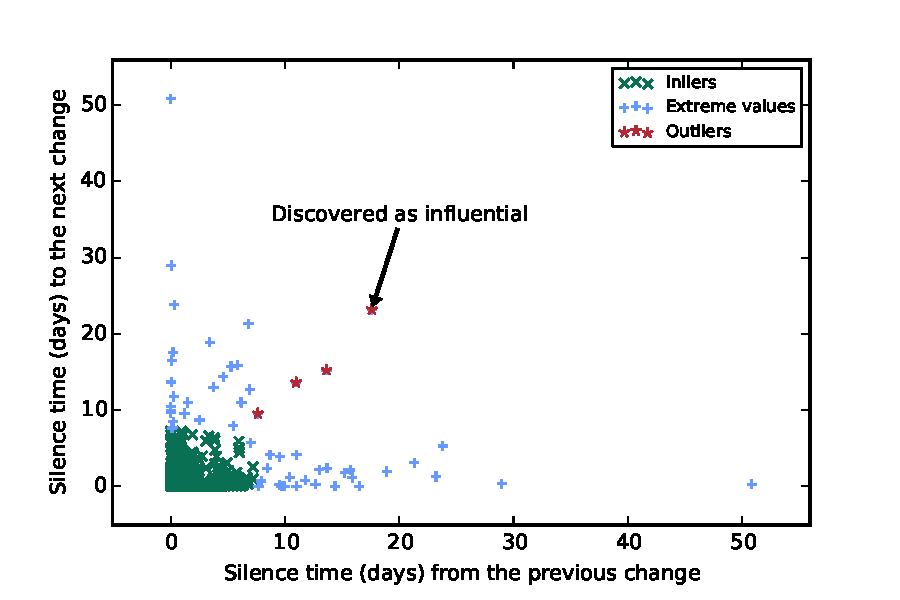
\includegraphics[width=0.8\linewidth]{fig/build-gradle.pdf}
\caption{Outlier detection to discover isolated commits for {\em build.gradle} file in {\tt Spring framework}.}
\label{fig:build-gradle}
\end{figure}


%\begin{table*}[t]
\centering
\caption{Isolated commits for ``StorageProxy.java'' in ``Cassandra'' project}
\begin{tabular}{|p{3cm}|p{1.5cm}|p{8cm}|}
\hline
File & Short hash & Commit message\\\hline
StorageProxy.java&97c022f&short circuits sending a message if the mutation's destination is the local node.  does not implement hint handling; takes the full message route if hints are involved.  patch by Sandeep Tata; reviewed by jbellis for CASSANDRA-132 \\\hline
StorageProxy.java&f6d0154&merge from 0.3 branch \\\hline
StorageProxy.java&3673e28&multitable support. \\\hline
StorageProxy.java&4e3a440&spelling fixes.  patch by Michael Greene; reviewed by jbellis for CASSANDRA-281 \\\hline
StorageProxy.java&dd1688c&merge from 0.4 branch \\\hline
StorageProxy.java&5e9b35c&rename getMessagingInstance -> instance; r/m unused methods from FBUtiltities patch by jbellis; reviewed by Eric Evans for CASSANDRA-385 \\\hline
StorageProxy.java&9cc51b5&fix range queries and Range/Bounds intersections.  patch by jbellis; tested by Jack Culpepper for CASSANDRA-781 \\\hline
StorageProxy.java&0095f0c&CASSANDRA-625 switch to slf4j logging. Patch by Gabriele Renzi, reviewed by Gary Dusbabek. \\\hline
StorageProxy.java&c5e97fd&improve DEBUG logging of insert path.  patch by Ryan King and jbellis for CASSANDRA-1023 \\\hline
StorageProxy.java&7c9191f&merge from 0.6 \\\hline
StorageProxy.java&d8755b3&clean up of TokenMetadata and ARS.  patch by mdennis; reviewed by jbellis for CASSANDRA-1194 \\\hline
StorageProxy.java&aa95d4a&always repair on digest mismatch for CL > 1.  patch by jbellis \\\hline
StorageProxy.java&389bac7&merge from 0.6 \\\hline
\end{tabular}
\label{tab:StorageProxy-isolated-commits}
\end{table*}


%For each project, we compile a list of isolated commits.  As an
%example, Table~\ref{tab:io-isolated-commits} shows all isolated
%commits in the ``commons-io'' project.



%\begin{table*}[t]
%\centering
%\caption{Isolated commits in ``commons-io'' project}
%\begin{tabular}{|p{5cm}|p{1.5cm}|p{6cm}|}
%\hline File & Short hash & Commit message\\\hline pom.xml & efcc1db &
%Fix IO-161 FileCleaningTrackerTestCase hangs - reported by Sebastiano
%Vigna \\\hline pom.xml & d9eb28f & Update to commons-parent-12
%\\\hline pom.xml & 1bad2ed & [IO-435] Document thrown
%IllegalArgumentException in FileUtils. Thanks to Dominik
%Stadler. \\\hline changes.xml & eabcac3 & IO-165 set svn:eol-style to
%native - thanks to Benjamin Bentmann for the patch \\\hline
%Tailer.java & e871a89 & IO-274 - Tailer returning partial lines when
%reaching EOF before EOL \\\hline RELEASE-NOTES.txt & 09780d1 & A note
%on the Lang 1.1 dependency. \\\hline RELEASE-NOTES.txt & 3dba7f1 &
%removed note about Lang dependency \\\hline RELEASE-NOTES.txt &
%947dc3d & svn:keywords correction \\\hline RELEASE-NOTES.txt & afbfd3c
%& Comprehensive release notes with history. \\\hline
%FilenameUtilsWildcardTestCase.java & 4aac0d0 & IO-167 Fix
%case-insensitive string handling - thanks to Benjamin Bentmann
%\\\hline project.xml & 49ffe91 & Remove jakarta references from m1 and
%m2 builds \\\hline tasks.xml & f852873 & added finding subsystem to IO
%along with WildcardUtils \\\hline STATUS.html & ade6c8c & Fix status
%info about releases \\\hline LockableFileWriterTest.java & aa9a1d0 &
%Remove extraneous exec properties \\\hline CopyUtils.java & 4ae1536 &
%IO-140 annotate with @Override and @Deprecated \\\hline
%\end{tabular}
%\label{tab:io-isolated-commits}
%\end{table*}

%Out of these 15 isolated, six of them obviously intend to fix issues.

%TODO: Analyze these isolated commits.


%\paragraph{Isolated changes for developers}

Individual project contributors also often exhibit abnormal
behaviors which may suggest influential code changes.
For instance, one core developer constantly contributes
 to a specific project. If such a developer
submits isolated commits (i.e., commits that are a long time away from
the author's previous commit as well as his/her next commit), this
might be recognized as an emergency case where immediate attention is needed. 

In this study, we also systematically classified isolated commits based on
developer behaviors as potentially influential. For example, from commits by
developer {\em Stefan Bodewig} in {\tt Commons-COMPRESS}, we found an isolated
commit\footnote{Commit \tt\small fadbb4cc0e9ca11c371c87ce042fd596b13eb092}
where he proposed a major bug fix for the implementation of the {\em
ZipArchiveEntry} API. Before this influential software change, any attempt to create a
zip file with a large number of entries was producing a corrupted file.

% \begin{figure}[t] \centering 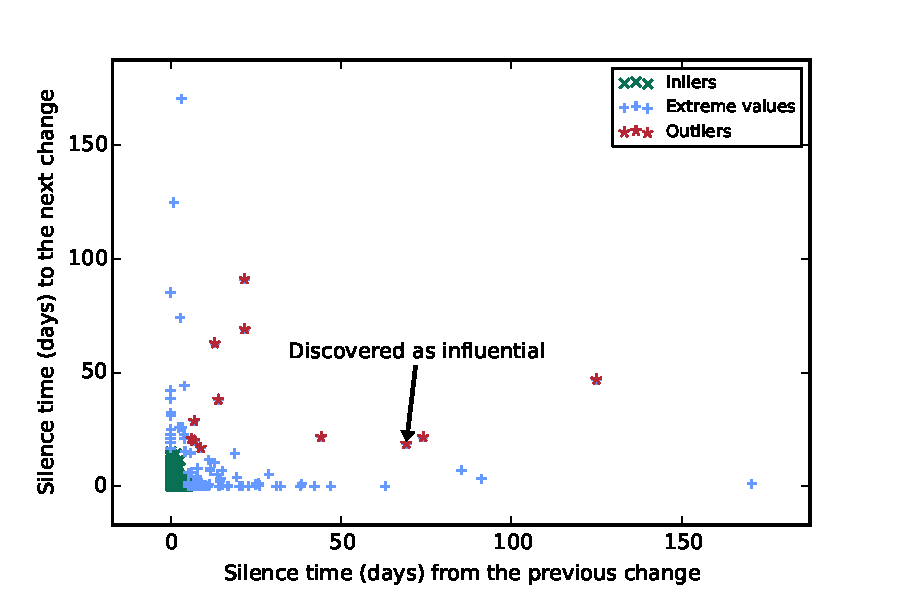
\includegraphics[width=\linewidth]{fig/bodewig.pdf}
% \caption{Outlier detection to discover isolated commits by {\em Stefan Bodewig}, 
% a {\tt Commons-COMPRESS} core contributor.}
% \label{fig:bodewig}
% \end{figure}

%\paragraph{Unexpected contributions by author}
%\tb{To be removed}
%Normally developers focus on a certain set of files in an open source
%project, as a result, each file tends to have a stable set of core
%contributors.  However, when a developer contributes to a file that is
%beyond his/her file set of routine responsibilities, this abnormality
%may suggest that the contribution is emergent or should go under
%scrutiny. In other words, it is potentially influential.



To confirm that an isolated change is influential we verify that 1) its importance is clearly stated in the change log and
2) the implication of the change for dependent modules and client applications is apparent.
Table~\ref{tab:isolated} provides the statistics on detected isolated commits
and the results of our manual analysis on those  commits to confirm influential changes.


\begin{table}[t]
\centering
\caption{Statistics of identified isolated commits and the associated manually confirmed influential changes.}
\centering
\resizebox{0.6\linewidth}{!}
{
\begin{tabular}{lcc}
    Project Name & \# isolated commits & \# influential changes\\
\toprule

{\tt Commons-codec} & 7 & 3 \\
{\tt Commons-collections} & 28 & 9 \\
{\tt Commons-compress} & 17 & 5 \\
{\tt Commons-csv} & 13 & 4 \\
{\tt Commons-io} & 18 & 5 \\
{\tt Commons-lang} & 22 & 7 \\
{\tt Commons-math} & 29 & 5 \\
{\tt Spring-framework} & 56 & 8 \\
{\tt Storm} & 48 & 7 \\
{\tt Wildfly} & 213 & 1 \\
\midrule
Total & 451 & 54 \\
\bottomrule

\end{tabular}
}

\label{tab:isolated}
\end{table}


\subsubsection{Changes referred to in other changes.}
We considered that popular changes are potentially influential.
These are changes that other developers have somehow noticed (e.g., incomplete fix,
API change that causes collateral evolution). Indeed,
when developers submit software changes to a project, they usually submit
also a commit message introducing what their patch does. Occasionally,
developers refer to others' contributions in these messages. This kind of
behaviors suggests that the referred contribution is influential, at
least to a certain extent. For example, in the {\tt Commons-CSV} project, 
commit\footnote{Commit \tt\small 93089b260cd2030d69b3f7113ed643b9af1adcaa} 
{\tt 93089b26} is referred by another commit\footnote{Commit \tt\small
05b5c8ef488d5d230d665b9d488ca572bec5dc0c}.
This commit implemented the capability to detect start of line, 
which is surely an influential change for the implementation of CSV format reading.

Because some of the projects have switched from
using Subversion to using Git, we first managed to create a mapping between
the Subversion revision numbers (which remain as such in the commit messages) and
the newly attributed Git Hash code. 
To confirm that a change referenced by other changes is influential we verify that 1) it is indeed referenced by 
others because it was inducing their changes, and 2) the implication of the change for dependent modules and client applications
are apparent. Table~\ref{tab:referenced} provides the
statistics of influential changes derived with this metric.


\begin{table}[t!]
\centering
\caption{Statistics of identified referenced commits and influential commits.}
\centering
\resizebox{0.8\linewidth}{!}
{
\begin{tabular}{lcc}
    Project Name & \# referenced commits & \# influential changes\\
\toprule

{\tt Commons-codec} & 8 & 3 \\
{\tt Commons-collections} & 3 & 1 \\
{\tt Commons-compress} & 3 & 0 \\
{\tt Commons-csv} & 3 & 2 \\
{\tt Commons-io} & 5 & 1 \\
{\tt Commons-lang} & 21 & 2 \\
{\tt Commons-math} & 43 & 3 \\
{\tt Spring-framework} & 1 & 1 \\
{\tt Storm} & 1 & 0 \\
{\tt Wildfly} & 11 & 9 \\
\midrule
Total & 99 & 22 \\
\bottomrule

\end{tabular}
}

\label{tab:referenced}
\end{table}


\subsection{Manual Validation on a Sample Set}

We then set to manually validate the suitability of the metrics used in our observational
study. 
To that end, we must compute the rate of influential changes among the changes that
exhibit high scores in the metrics defined about, as well as the rate of influential changes
among a randomly selected set of changes within a project history.
Concretely, we manually verify whether the potential influential changes yielded by the
systematic analysis are indeed acceptable as influential (240, 451, and 99 commits shown 
in Tables~\ref{tab:blocking}, \ref{tab:isolated}, 
and~\ref{tab:referenced}, respectively -- i.e., 785 distinct commits as shown in Table~\ref{tab:qualitative}). 
We further randomly pick change commits from each project
and manually check the percentage of changes that can be accepted as influential as well. The
comparison between the two types of datasets aimed at validating our choices
of post-mortem metrics to easily collect influential changes.
Table~\ref{tab:qualitative} provides results of the qualitative assessment.
For each project, the random dataset size is fixed to 20 commits\footnote{We selected this number to align with the smallest number of commits found using the systematic analysis technique on a project}, leading to a
manual checking of 200 changes. Our systematic analysis findings produce
change datasets with highest rates of ``truly'' influential changes (an order
of magnitude more than what can be identified in random samples).

The validation procedure, for a commit to be accepted as influential, was implemented to follow a simple but rigorous procedure. Given a commit,
we first read the commit log to understand ``what'' the change is about. At this point, we look for
hints that the change is influential (e.g., the commit author can suggest it when he enumerates the
important issue that the change addresses). Second, we look at the component that the commit touches as well
as the amount of changes that are made in the commit (e.g., an entire repackaging of a codec code with a
new build configuration may be too invasive and requests several changes later, including a potential reverting). Finally, we consider the commit number as well as key terms that we identify in the commit log, and grep other
subsequent commits to check whether other commits were necessary follow-up of the commit under study, and thus
to measure its 'influence' on the development.

\begin{table}[t] 
\centering 
\caption{Manual assessment results. We
compared the percentage of changes that were manually confirmed to be
influential from the datasets yielded by our systematic analysis (see Section~\ref{sec:systemanalysis}) and a random
selection in projects. Note that we count unique commits in this table, since 
some commits fall into more than one categories.}
%\multirow{2}{*}{Safety hole} & \multicolumn{2}{c}{Number of exported functions collected in the } \\
\centering
\resizebox{0.8\linewidth}{!}
{
\begin{tabular}{l c c c | c c  c}
  \multirow{2}{*}{\bf Project Name} & 
  \multicolumn{3}{c|}{\bf Systematic Analysis Findings} & 
  \multicolumn{3}{c}{\bf Random Selection} \\
  & Total & Influential & Rate & Total & Influential & Rate \\

\toprule

{\tt Commons-codec} & 40 & 8 & 20.0\% & 20 & 0 & 0.0\% \\
{\tt Commons-collections} & 42 & 17 & 40.5\% & 20 & 0 & 0.0\%\\
{\tt Commons-compress} & 27 & 9 & 33.3\% & 20 & 1 & 5.0\% \\
{\tt Commons-csv} & 21 & 11 & 52.4\% & 20 & 1 & 5.0\% \\
{\tt Commons-io} & 33 & 6 & 18.2\% & 20 & 0 & 0.0\%\\
{\tt Commons-lang} & 72 & 24 & 33.3\% &20 & 0 & 0.0\%\\
{\tt Commons-math} & 108 & 14 & 13.0\% &20 &  0 & 0.0\%\\
{\tt Spring-framework} & 110 & 51 & 46.4\% &  20 & 1& 5.0\%\\
{\tt Storm} & 89 & 10 & 11.2\% & 20 & 1 & 5.0\% \\
{\tt Wildfly} & 243 & 27 & 11.1\% & 20 & 1 & 5.0\% \\
\midrule
Total & 785 & 177 & {\bf 22.5\%} & 200 & 5 & {\bf 2.5\%}\\
\bottomrule

\end{tabular}}

\label{tab:qualitative}
\end{table}

%\begin{center}
%    \setlength{\fboxsep}{5pt}%
%    \Ovalbox{%
%        \begin{minipage}{.42\textwidth}
%            \begin{center}
{\bf Conclusion:}{\it 
The difference in influential rate values with random shows that our 
post-mortem metrics (isolated changes, popular commits, changes unlocking issues) are indeed 
good indicators for collecting \underline{some} influential software changes.
                }
%            \end{center}
%    \end{minipage}}
%\end{center}
% \begin{center}
% \begin{longtable}{|p{6.7cm}|p{6.7cm}|}
% \toprule
% \bfseries Hash & \bfseries Refers to\\
% \midrule \endhead
% \bottomrule \endfoot
% \csvreader[late after line=\\\hline]
% {referenced.commits/camel.csv}{}{\csvlinetotablerow}
% \caption{Commit references in ``camel'' project.}
% \label{tab:ref-commit-camel}
% \end{longtable}
% \end{center}
